\begin{enumerate}[label=\thesection.\arabic*,ref=\thesection.\theenumi]
\numberwithin{equation}{enumi}
\numberwithin{figure}{enumi}
\numberwithin{table}{enumi}
\item In the Figure \ref{fig:9/9/2/1}, $ABCD$ is a parallelogram, $AE \perp DC$ and $CF \perp AD$. If $AB = 16 cm$, $AE = 8 cm$, and $CF = 10cm$, find $AD$.
	\begin{figure}[!h]
		\centering
 \includegraphics[width=\columnwidth]{chapters/9/9/2/1/figs/fig1.pdf}
		\caption{}
		\label{fig:9/9/2/1}
  	\end{figure}
\iffalse
\documentclass[journal,12pt,twocolumn]{IEEEtran}

\usepackage[utf8]{inputenc}
\usepackage{kvmap}
\usepackage{graphics} 

\usepackage{setspace}
\usepackage{gensymb}

\singlespacing

\usepackage{amsthm}

\usepackage{mathrsfs}
\usepackage{txfonts}
\usepackage{stfloats}
\usepackage{bm}
\usepackage{cite}
\usepackage{cases}
\usepackage{subfig}

\usepackage{longtable}
\usepackage{multirow}

\usepackage{enumitem}
\usepackage{mathtools}
\usepackage{steinmetz}
\usepackage{tikz}
\usepackage{circuitikz}
\usepackage{verbatim}
\usepackage{tfrupee}
\usepackage[breaklinks=true]{hyperref}
\usepackage{graphicx}
\usepackage{tkz-euclide}
\usepackage{float}

\usetikzlibrary{calc,math}
\usepackage{listings}
    \usepackage{color}                                            %%
    \usepackage{array}                                            %%
    \usepackage{longtable}                                        %%
    \usepackage{calc}                                             %%
    \usepackage{multirow}                                         %%
    \usepackage{hhline}                                           %%
    \usepackage{ifthen}                                           %%
    \usepackage{lscape}     
\usepackage{multicol}
\usepackage{chngcntr}

\DeclareMathOperator*{\Res}{Res}

\renewcommand\thesection{\arabic{section}}
\renewcommand\thesubsection{\thesection.\arabic{subsection}}
\renewcommand\thesubsubsection{\thesubsection.\arabic{subsubsection}}

\renewcommand\thesectiondis{\arabic{section}}
\renewcommand\thesubsectiondis{\thesectiondis.\arabic{subsection}}
\renewcommand\thesubsubsectiondis{\thesubsectiondis.\arabic{subsubsection}}

\hyphenation{op-tical net-works semi-conduc-tor}
\def\inputGnumericTable{}                                 %%

\lstset{
%language=C,
frame=single, 
breaklines=true,
columns=fullflexible
}
\begin{document}

\newtheorem{theorem}{Theorem}[section]
\newtheorem{problem}{Problem}
\newtheorem{proposition}{Proposition}[section]
\newtheorem{lemma}{Lemma}[section]
\newtheorem{corollary}[theorem]{Corollary}
\newtheorem{example}{Example}[section]
\newtheorem{definition}[problem]{Definition}

\newcommand{\BEQA}{\begin{eqnarray}}
\newcommand{\EEQA}{\end{eqnarray}}
\newcommand{\define}{\stackrel{\triangle}{=}}
\newcommand\hlight[1]{\tikz[overlay, remember picture,baseline=-\the\dimexpr\fontdimen22\textfont2\relax]\node[rectangle,fill=blue!50,rounded corners,fill opacity = 0.2,draw,thick,text opacity =1] {$#1$};}
\bibliographystyle{IEEEtran}
\providecommand{\mbf}{\mathbf}
\providecommand{\pr}[1]{\ensuremath{\Pr\left(#1\right)}}
\providecommand{\qfunc}[1]{\ensuremath{Q\left(#1\right)}}
\providecommand{\sbrak}[1]{\ensuremath{{}\left[#1\right]}}
\providecommand{\lsbrak}[1]{\ensuremath{{}\left[#1\right.}}
\providecommand{\rsbrak}[1]{\ensuremath{{}\left.#1\right]}}
\providecommand{\brak}[1]{\ensuremath{\left(#1\right)}}
\providecommand{\lbrak}[1]{\ensuremath{\left(#1\right.}}
\providecommand{\rbrak}[1]{\ensuremath{\left.#1\right)}}
\providecommand{\cbrak}[1]{\ensuremath{\left\{#1\right\}}}
\providecommand{\lcbrak}[1]{\ensuremath{\left\{#1\right.}}
\providecommand{\rcbrak}[1]{\ensuremath{\left.#1\right\}}}
\theoremstyle{remark}
\newtheorem{rem}{Remark}
\newcommand{\sgn}{\mathop{\mathrm{sgn}}}
\providecommand{\abs}[1]{\left\vert#1\right\vert}
\providecommand{\res}[1]{\Res\displaylimits_{#1}} 
\providecommand{\norm}[1]{$\left\lVert#1\right\rVert$}
%\providecommand{\norm}[1]{\lVert#1\rVert}
\providecommand{\mtx}[1]{\mathbf{#1}}
\providecommand{\mean}[1]{E\left[ #1 \right]}
\providecommand{\fourier}{\overset{\mathcal{F}}{ \rightleftharpoons}}
%\providecommand{\hilbert}{\overset{\mathcal{H}}{ \rightleftharpoons}}
\providecommand{\system}{\overset{\mathcal{H}}{ \longleftrightarrow}}
	%\newcommand{\solution}[2]{\textbf{Solution:}{#1}}
\newcommand{\solution}{\noindent \textbf{Solution: }}
\newcommand{\cosec}{\,\text{cosec}\,}
\providecommand{\dec}[2]{\ensuremath{\overset{#1}{\underset{#2}{\gtrless}}}}
\newcommand{\myvec}[1]{\ensuremath{\begin{pmatrix}#1\end{pmatrix}}}
\newcommand{\mydet}[1]{\ensuremath{\begin{vmatrix}#1\end{vmatrix}}}
\numberwithin{equation}{subsection}
\makeatletter
\@addtoreset{figure}{problem}
\makeatother
\let\StandardTheFigure\thefigure
\let\vec\mathbf
\renewcommand{\thefigure}{\theproblem}
\def\putbox#1#2#3{\makebox[0in][l]{\makebox[#1][l]{}\raisebox{\baselineskip}[0in][0in]{\raisebox{#2}[0in][0in]{#3}}}}
     \def\rightbox#1{\makebox[0in][r]{#1}}
     \def\centbox#1{\makebox[0in]{#1}}
     \def\topbox#1{\raisebox{-\baselineskip}[0in][0in]{#1}}
     \def\midbox#1{\raisebox{-0.5\baselineskip}[0in][0in]{#1}}
\vspace{3cm}
\title{\textbf{Matrices Assignment - Line} }
\author{Dukkipati Vijay Sai}
\maketitle
\newpage
\bigskip
\renewcommand{\thefigure}{\theenumi}
\renewcommand{\thetable}{\theenumi}
Get Python code for the figure from 
\begin{lstlisting}
https://github.com/dukkipativijay/Fwciith2022/tree/main/Assignment%201/Codes/src
\end{lstlisting}
Get LaTex code from
\begin{lstlisting}
https://github.com/dukkipativijay/Fwciith2022/tree/main/Assignment%201%20-%20Assembly/Codes
\end{lstlisting}
%
\section{Question}
\centering
\textbf{\textit{Class 9, Exercise 9.2, Q(1)}}\\
\vspace{0.25cm}
\raggedright
\fi
	\iffalse
	\solution Let 
	\begin{align}
		\vec{D} = \vec{0}.
	\end{align}
	Then, from the given information
	\begin{align}
		\vec{e}_2^{\top}\vec{A} = 8 &= h_1
		\\
		\implies 
		\vec{A} =h_1\vec{e}_2 &+ \mu \vec{e}_1
		\label{eq:9/9/2/1/1}
		\\
		\vec{C} =  16\vec{e}_2 &= a\vec{e}_2
		\label{eq:9/9/2/1/2}
		\\
		\norm{\vec{C}-\vec{F}} = 10 &= h_2
		\label{eq:9/9/2/1/3}
		\\
		\brak{\vec{C}-\vec{F}}^{\top}\vec{A} &= \vec{0}
		\\
		\implies \vec{F} &=\vec{C}+ \mu_2\vec{R}\vec{A}
		\label{eq:9/9/2/1/4}
	\end{align}
	where $\\mu_1, \mu_2$ are unknown and $\vec{R}$ defined in Appendix 
	\ref{prop:mat/rot/pi/2}. Substituting from 
		\eqref{eq:9/9/2/1/4}
		in
		\eqref{eq:9/9/2/1/3},
	\begin{align}
		\norm{\vec{C}-\vec{F}}^2 &= h_2^2
		\\
		\implies 
		\mu_2^2	\norm{\vec{A}}^2&= h_2^2 \quad \brak{\because \vec{R}^{\top}\vec{R}= \vec{I}}
	\end{align}
	From 
		\eqref{eq:9/9/2/1/1}, 
	\begin{align}
		\norm{\vec{A}}^2 &= h_1^2 + \mu_1^2
		\\
		\implies \frac{h_2^2}{{\mu_2}^2} &= h_1^2 + \mu_1^2
		\\
		\text{or, }\mu_1  = 
	\end{align}
\centering
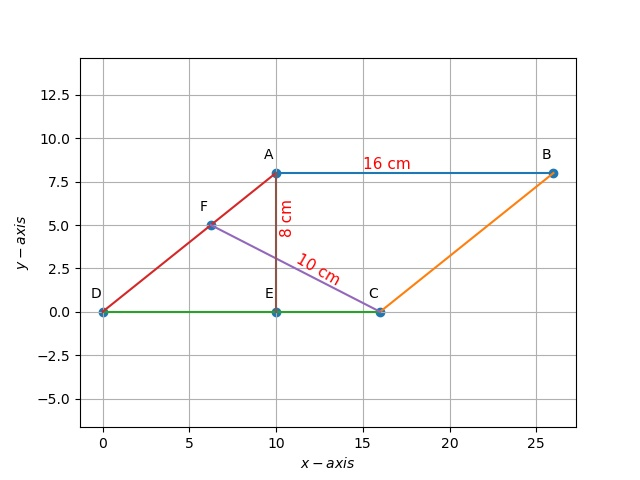
\includegraphics[width=0.5\textwidth]{fig 1.jpeg}
Figure 1 - Parallelogram ABCD


\section{Construction}
\vspace{0.5cm}
\begin{tabular}{|c|c|c|}
\hline
Symbol & Value & Description\\
\hline
D & Origin (0,0) & Vertex D \\
\hline
AB & 16cm & $\|\hspace{0.1cm} \vec{B} - \vec{A} \hspace{0.1cm}\|$ \\
\hline
CD & 16cm & $\|\hspace{0.1cm} \vec{D} - \vec{C} \hspace{0.1cm}\| = \|\hspace{0.1cm} \vec{B} - \vec{A} \hspace{0.1cm}\|$ \\
\hline
C & (16,0) & Vertex C ($\because CD = 16cm$)\\
\hline
AE & 8cm & $\|\hspace{0.1cm} \vec{E} - \vec{A} \hspace{0.1cm}\|$ \\
\hline

\end{tabular}
\begin{tabular}{|c|c|c|}

\hline
CF & 10cm & $\|\hspace{0.1cm} \vec{F} - \vec{C} \hspace{0.1cm}\|$ \\
\hline

A & (10,8) & Ay = Dy + $|\overrightarrow{AE}|$\\
 & & $Ax = \sqrt{\frac{CF^2}{AB^2 - CF^2}}$\\
 
\hline

B & (26,8) & By = Dy + $|\overrightarrow{AE}|$\\
 & & $Bx = Ax + AB$\\
 
\hline
F & (6.25,5) & $Fy = 0.8 \hspace{0.1cm} X\hspace{0.1cm} Fx$\\
\hline

E & (10,0) & Ex = Ax, Ey=0 \\
\hline

\end{tabular}


\section{Solution}
\raggedright
From the properties of Parallelogram we know that, Opposite sides are equal in length. Hence, we can write,\\
\vspace{0.25cm}
\centering
$|\hspace{0.1cm}\overrightarrow{CD}\hspace{0.1cm}| = |\hspace{0.1cm}\overrightarrow{AB}\hspace{0.1cm}|$\\
\vspace{0.25cm}
Hence,
$\|\hspace{0.1cm} \vec{D} - \vec{C} \hspace{0.1cm}\|\hspace{0.1cm} = \hspace{0.1cm} \|\hspace{0.1cm} \vec{B} - \vec{A}\hspace{0.1cm} \|\hspace{0.1cm}=\hspace{0.1cm}16cm$\\
\vspace{0.25cm}
\raggedright
We also know that,\\
\vspace{0.25cm}
\centering
Area of a Parallelogram = Base x Height\\
\vspace{0.25cm}
\raggedright
Since, it is given that $\overrightarrow{AE} \perp \overrightarrow{CD}$  from the figure 1 we can write,\\
\vspace{0.25cm}
Area of Parallelogram ABCD = $|\hspace{0.1cm} \overrightarrow{CD}\hspace{0.1cm}|\hspace{0.1cm} x\hspace{0.1cm}|\hspace{0.1cm}  \overrightarrow{AE}\hspace{0.1cm}|$ \hspace{0.1cm} (1)\\
\vspace{0.25cm}
\hspace{4.5cm} $=\hspace{0.1cm} \|\hspace{0.1cm} \vec{D} - \vec{C} \hspace{0.1cm}\|\hspace{0.1cm} x\hspace{0.1cm} \|\hspace{0.1cm} \vec{E} - \vec{A}\hspace{0.1cm} \|$\\
\vspace{0.25cm}
But it is also given that $\overrightarrow{CF} \perp \overrightarrow{AD}$. Hence we can similarly write,\\
\vspace{0.25cm}
Area of Parallelogram ABCD = $|\hspace{0.1cm} \overrightarrow{AD}\hspace{0.1cm}|\hspace{0.1cm}  x\hspace{0.1cm}|\hspace{0.1cm}  \overrightarrow{CF}\hspace{0.1cm}|$ \hspace{0.1cm} (2)\\
\vspace{0.25cm}
\hspace{4.5cm} $=\hspace{0.1cm} \|\hspace{0.1cm} \vec{D} - \vec{A} \hspace{0.1cm}\|\hspace{0.1cm} x\hspace{0.1cm} \|\hspace{0.1cm} \vec{F} - \vec{C}\hspace{0.1cm} \|$\\
\vspace{0.25cm}
Observing Eq. (1) and Eq. (2), we see that both are equal. Hence we get,\\
\vspace{0.25cm}
\centering

$ \|\hspace{0.1cm} \vec{D} - \vec{C} \hspace{0.1cm}\|\hspace{0.1cm} x\hspace{0.1cm} \|\hspace{0.1cm} \vec{E} - \vec{A}\hspace{0.1cm} \|\hspace{0.1cm} = \hspace{0.1cm} \|\hspace{0.1cm} \vec{D} - \vec{A} \hspace{0.1cm}\|\hspace{0.1cm} x\hspace{0.1cm} \|\hspace{0.1cm} \vec{F} - \vec{C}\hspace{0.1cm} \|  $

\vspace{0.25cm}

$|\hspace{0.1cm} 16\hspace{0.1cm}|\hspace{0.1cm}  x\hspace{0.1cm}|\hspace{0.1cm}  8 \hspace{0.1cm}|= \hspace{0.1cm}  \|\hspace{0.1cm} \vec{D} - \vec{A} \hspace{0.1cm}\| \hspace{0.1cm} x\hspace{0.1cm} |\hspace{0.1cm} 10\hspace{0.1cm}|$\\

\vspace{0.25cm}

128 = $\hspace{0.1cm} \|\hspace{0.1cm} \vec{D} - \vec{A} \hspace{0.1cm}\|\hspace{0.1cm}$ x 10\\

\vspace{0.25cm}

$ \|\hspace{0.1cm} \vec{D} - \vec{A} \hspace{0.1cm}\| \hspace{0.1cm}=\hspace{0.1cm}\frac{128}{10}$\\

\vspace{0.25cm}

$\therefore$ $|\hspace{0.1cm}$\textbf{$\overrightarrow{\vec{AD}}\hspace{0.1cm} |$ = 12.8 cm}\\

\vspace{0.25cm}

\centering
\textbf{Hence, This is the required value of AD.}

\vspace{0.25cm}


\end{document}
Footer
\fi

\item For a given Parallelogram $ABCD$, show that for any
point $\vec{P}$ inside the parallelogram,
\begin{enumerate}
	\item $Ar(APD)+Ar(PBC) = \frac{1}{2}Ar(ABCD)$
	\item $Ar(APD)+Ar(PBC) = Ar(APB)+Ar(PCD)$
\end{enumerate}
\iffalse
\documentclass[journal,10pt,twocolumn]{article}
\usepackage{graphicx}
\graphicspath{{./Figures/}}
\usepackage[margin=0.5in]{geometry}
\usepackage[cmex10]{amsmath}
\usepackage{amssymb}
\usepackage{array}
\usepackage{booktabs}

\title{\textbf{Line Assignment}}
\author{Bole Manideep}
\date{September 2022}

\providecommand{\norm}[1]{\left\lVert#1\right\rVert}
\providecommand{\abs}[1]{\left\vert#1\right\vert}
\let\vec\mathbf
\newcommand{\myvec}[1]{\ensuremath{\begin{pmatrix}#1\end{pmatrix}}}
\newcommand{\mydet}[1]{\ensuremath{\begin{vmatrix}#1\end{vmatrix}}}
\providecommand{\brak}[1]{\ensuremath{\left(#1\right)}}

\begin{document}
\maketitle
\fi

	\begin{figure}[!h]
		\centering
 \includegraphics[width=\columnwidth]{chapters/9/9/2/4/figs/Question.png}
		\caption{}
		\label{fig:9/9/2/4}
  	\end{figure}
	\iffalse
\begin{figure}[h]
\centering
\includegraphics[width=1\columnwidth]{Question.png}
\caption{Parallelogram ABCD with interior point P}
\label{fig:Parallelogram}
\end{figure}

\section*{Solution}

\subsection*{Part 1}
WKT, area of a parallelogram with adjacent sides a \& b is,
\begin{equation}
\text{Area of parallelogram = } \norm{\vec{a} \times \vec{b}}
\label{eq-1-}
\end{equation}
And, area of a triangle with adjacent sides p \& q is,
\begin{equation}
\text{Area of triangle = } \frac{1}{2} \norm{\vec{p} \times \vec{q}}
\label{eq-2-}
\end{equation}
From Figure 1,\\ $\vec{(A-D)}\hspace{2mm}\&\hspace{2mm}\vec{(B-C)}$ are equal,\\
\begin{equation}
\norm{\vec{A-D}} = \norm{\vec{B-C}}
\label{eq-3-}
\end{equation}
Consider $\triangle$APD
\begin{equation}
\text{Area of } \triangle APD = \frac{1}{2}\norm{\vec{(A-D)} \times \vec{(A-P)}}
\label{eq-4-}
\end{equation}
Consider $\triangle$PBC
\begin{equation}
\text{Area of } \triangle BPC =  \frac{1}{2}\norm{\vec{(B-C)} \times \vec{(P-B)}}
\label{eq-5-}
\end{equation}
On adding \eqref{eq-4-} \& \eqref{eq-5-},
\begin{multline}
Ar(APD) + Ar(PBC) =\\
 \frac{1}{2}\norm{\vec{(A-D)} \times \vec{(A-P)}} + \frac{1}{2}\norm{\vec{(B-C)} \times \vec{(P-B)}}
\label{eq-6-}
\end{multline}
From equation \eqref{eq-3-},
\begin{multline}
Ar(APD) + Ar(PBC) =\\
 \frac{1}{2}\norm{\vec{(A-D)} \times \vec{(A-P)}} + \frac{1}{2}\norm{\vec{(A-D)} \times \vec{(P-B)}}
\label{eq-7-}
\end{multline}
\begin{multline}
\implies Ar(APD) + Ar(PBC) =\\ \frac{1}{2}\norm{\vec{(A-D)}\times[\vec{(A-P)} + \vec{(P-B)}]}
\label{eq-8-}
\end{multline}
Here, AP \& PB are adjacent sides of $\triangle$ APB
\\From Triangle law of vector addition, \\ $\vec{(A-P)} + \vec{(P-B)} = \vec{(A-B)}$
\begin{equation}
\implies Ar(APD) + Ar(PBC) = \frac{1}{2}\norm{\vec{(A-D)}\times\vec{(A-B)}}
\label{eq-9-}
\end{equation}
Since, $\vec{(A-D)} \hspace{2mm} \& \hspace{2mm} 1\vec{(A-B)}$ are adjacent sides of paralleogram ABCD
\\With reference to \eqref{eq-2-},
\begin{equation}
Ar(ABCD) = \norm{\vec{(A-D)}\times\vec{(A-B)}}
\label{eq-10-}
\end{equation}
From \eqref{eq-9-} \& \eqref{eq-10-}
\begin{equation}
\therefore \hspace{3mm} Ar(APD)+Ar(PBC) = \frac{1}{2}Ar(ABCD)
\label{eq-11-}
\end{equation}

\subsection*{Part 2}
Similarly, we can prove taht,
\begin{equation}
Ar(APB)+Ar(PBD) = \frac{1}{2}Ar(ABCD)
\label{eq-12-}
\end{equation}
On Comparing \eqref{eq-11-} and \eqref{eq-12-},
\begin{equation}
Ar(APD)+Ar(PBC) = Ar(APB)+Ar(PCD)
\label{eq-13-}
\end{equation}
\begin{center}
Hence Proved
\end{center}
\section*{Construction}
\raggedright A parallelogram ABCD is constructed unsing python,with the parameters that are mentioned in the table below.
\vspace{5mm}
\begin{center}
    \setlength{\arrayrulewidth}{0.1mm}
	\setlength{\tabcolsep}{12pt}
	\renewcommand{\arraystretch}{1.5}
\begin{tabular}{|c|c|c|}
	\hline 
    \textbf{Symbol} & \textbf{Value} & \textbf{Description}\\ 		\hline
    a & 4 & AB \\ \hline
    b & 2 & AD \\ \hline
    $\theta$ & 60$^{\circ}$ & $\angle$A \\ \hline
    $\vec{A}$ & $\myvec{0 \\ 0}$ & Vertex A \\ \hline
    $\vec{B}$ & $\myvec{a \\ 0}$ & Vertex B \\ \hline
    $\vec{D}$ & $b\myvec{\cos\theta \\ \sin\theta}$ & Vertex B \\ \hline
    $\vec{C}$ & $\vec{B+D}$ & Vertex C \\ \hline
    
\end{tabular}\\ \vspace{2mm}
Table 1: Parameter's Table
\end{center}

\section*{Proofs}
Triangle law of vector addition \\
Consider a triangle APB with vertices, \\ \vspace{2mm}
$\vec{A} = \myvec{0 \\ 0}$ \hspace{2mm}
$\vec{P} = \myvec{2 \\ 1}$ \hspace{2mm}
$\vec{B} = \myvec{0 \\ 4}$ \\ \vspace{2mm}
 
Vectors $\vec{(A-P)}, \vec{(P-B)} \hspace{1mm} \& \hspace{1mm} \vec{(A-B)} \hspace{1mm} are \hspace{1mm} sides \hspace{1mm} of \hspace{1mm} \triangle APB$\\
Let's consider,
\begin{equation}
\vec{(A-P)} + \vec{(P-B)} = \myvec{0 \\ 0} - \myvec{2 \\ 1} \hspace{2mm} + \hspace{2mm} \myvec{2 \\ 1} - \myvec{0 \\ 4}
\end{equation}
\begin{equation}
\implies \vec{(A-P)} + \vec{(P-B)} = \myvec{-2 \\ -1} \hspace{2mm} + \hspace{2mm} \myvec{2 \\ -3}
\end{equation}
\begin{equation}
\implies \vec{(A-P)} + \vec{(P-B)} = \myvec{0 \\ -4}
\end{equation}
\begin{equation}
\implies \vec{(A-P)} + \vec{(P-B)} = \myvec{0 \\ 0} - \myvec{0 \\ 4}
\end{equation} \vspace{1mm}
\begin{equation}
\therefore \vec{(A-P)} + \vec{(P-B)} = \vec{(A-B)}
\end{equation}  \\
\vspace{2mm}Thus, Triangle law of vector addition says taht sum of two adjacent side vectors of a triangle is equal to third side vector but in opposite direction.

\end{document}
\fi

\item In Fig.
		\ref{fig:9/9/2/5},
$PQRS$ and $ABRS$ are parallelograms
and $\vec{X}$ is any point on side $BR$. Show that  
\begin{enumerate}
    \item $ar (PQRS) = ar(ABRS)$
	    \label{prop:9/9/2/5}
    \item $ar(AXS) = \frac{1}{2} ar(PQRS)$
\end{enumerate}
	\begin{figure}[!h]
		\centering
 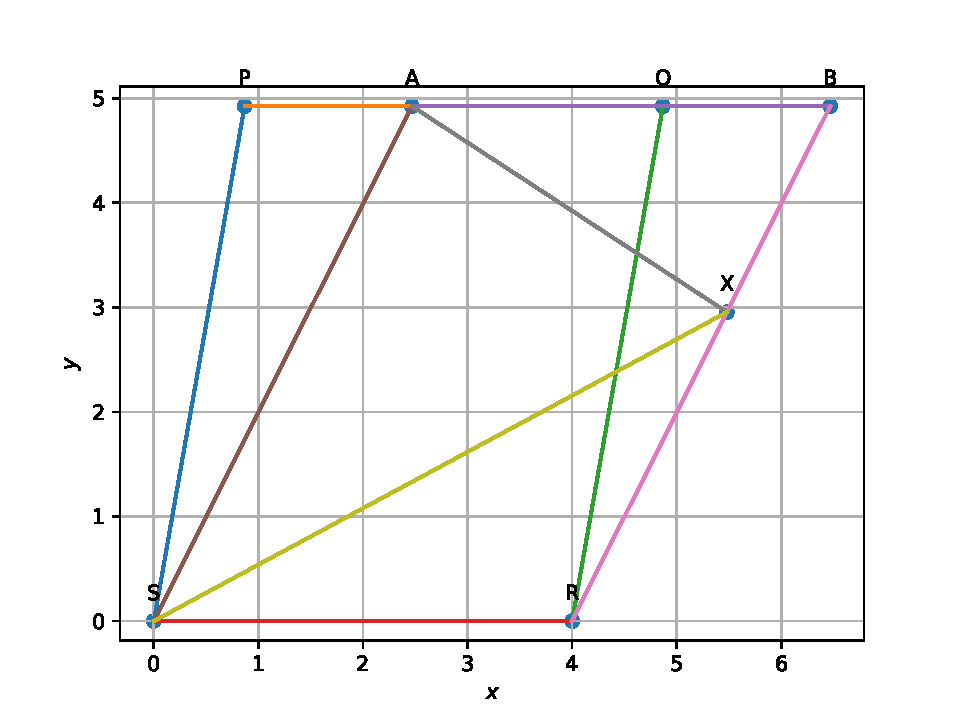
\includegraphics[width=\columnwidth]{chapters/9/9/2/5/figs/parallelogram1.pdf}
		\caption{}
		\label{fig:9/9/2/5}
  	\end{figure}
\iffalse
\documentclass{article}

% Language setting
% Replace `english' with e.g. `spanish' to change the document language
\usepackage[english]{babel}

% Set page size and margins
% Replace `letterpaper' with `a4paper' for UK/EU standard size
\usepackage[letterpaper,top=2cm,bottom=2cm,left=3cm,right=3cm,marginparwidth=1.75cm]{geometry}
% Useful packages
\usepackage{multicol}
\usepackage{amsmath}
\usepackage{amssymb}
\usepackage{graphicx}
\usepackage[framemethod=tikz]{mdframed}
\usepackage{array}
\usepackage{blindtext}
%\usepackage[paperwidth=10cm]{geometry}
\usepackage{tkz-euclide}
%\usepackage{tikz}
\usetikzlibrary{
  circuits.logic,
  circuits.logic.US,
  positioning
}

\usepackage[colorlinks=true, allcolors=blue]{hyperref}

\title{Line Assignment}
\author{Anusha Jella}
\begin{document}
\maketitle
\begin{multicols}{2}
	\fi
	\begin{proof}
		\begin{enumerate}
			\item 
		From Appendix
	  \ref{eq:two-pgm},
  \begin{align}
 \vec{A}-\vec{B} = \vec{S} -\vec{R} = \vec{P}-\vec{Q}
		\label{eq:9/9/2/5/1}
  \end{align}
  and from Appendix
  \ref{prop:pgm2d}, using 
		\eqref{eq:9/9/2/5/1}, we obtain Property
	    \ref{prop:9/9/2/5}.
    \item Using section formula, let 
  \begin{align}
	\vec{X} =   \frac{\vec{R}+k\vec{B}}{1+k}.
  \end{align}
  Then, 
  \begin{align}
	  ar\brak{AXS} &= \frac{1}{2} \norm{	\vec{S}\times\vec{X}+\vec{X}\times \vec{A}+\vec{A}\times \vec{S}}
	  \\
	  &= \frac{1}{2} \norm{	\frac{\vec{S}\times\vec{R}+k\vec{S}\times \vec{B}+\vec{R}\times \vec{A}+k\vec{B}\times \vec{A}}{k+1}+\vec{A}\times \vec{S}}
  \end{align}
  Substituting for $\vec{B}$ from 
		\eqref{eq:9/9/2/5/1}
		in the above,
  \begin{align}
	  ar\brak{AXS} &= \frac{1}{2} \norm{	\frac{\vec{S}\times\vec{R}+\vec{R}\times \vec{A}+k\brak{\vec{S}-\vec{A}}\times \brak{\vec{A}-\vec{S}+\vec{R}}}{k+1}+\vec{A}\times \vec{S}}
	  \\
&= \frac{1}{2} \norm{	\frac{\vec{S}\times\vec{R}+\vec{R}\times \vec{A}+k\brak{\vec{S}-\vec{A}}\times \vec{R}}{k+1}+\vec{A}\times \vec{S}}
\\
&= \frac{1}{2} \norm{	\vec{S}\times\vec{R}+\vec{R}\times \vec{A}+\vec{A}\times \vec{S}}
\\
	  &= \frac{1}{2}ar\brak{ABRS}
  \end{align}
		\end{enumerate}

	\end{proof}
	\iffalse
%\begin{figure}[h]
\centering
\includegraphics[width=\columnwidth] 
\centering{Fig 1. Parallelogram}
\label{fig:triangle}
%\end{figure}

\section*{\textbf{Solution 1:}}
\begin{flushleft}
Two parallelograms PQRS and ABRS, on the same base SR and between the same parallels PB and SR are given (see Fig.1).\\
We need to prove that ar(PQRS) = ar(ABRS).\\
Let, In PQRS 
\end{flushleft}
\begin{align}
           \boldsymbol{S}-\boldsymbol{R}&=\boldsymbol{p1}\hfill \\
           \boldsymbol{S}-\boldsymbol{P}&=\boldsymbol{p2}\hfill \\
           \boldsymbol{P}-\boldsymbol{Q} &=\boldsymbol{q1}\hfill \\
           \boldsymbol{R}-\boldsymbol{Q}&=\boldsymbol{q2}
\end{align}
 According to parrallelogram condition \\
\begin{align}
\lVert{\textbf{p1}}\rVert =\lVert{\textbf{q1}}\rVert \&\& \lVert{\textbf{p2}}\rVert =\lVert{\textbf{q2}}\rVert
\end{align}
\hspace{-4cm}Let,In ABRS
\begin{align}
           \boldsymbol{S}-\boldsymbol{R}&=\boldsymbol{s1} \hfill \\
           \boldsymbol{S}-\boldsymbol{A}&=\boldsymbol{s2} \hfill \\
           \boldsymbol{A}-\boldsymbol{B}&=\boldsymbol{r1} \hfill \\
           \boldsymbol{R}-\boldsymbol{B}&=\boldsymbol{r2}
\end{align} 
\hspace{-1cm}According to parallelogram condition 
\begin{align}
\lVert{\textbf{s1}}\rVert &=\lVert{\textbf{r1}}\rVert \&\& \lVert{\textbf{s2}}\rVert =\lVert{\textbf{r2}}\rVert
\end{align}
\hspace{-2cm}Area of parallelogram PQRS
\begin{align}
\boldsymbol{p1} X \boldsymbol{p2}       
\end{align}        
\hspace{-1cm}Now, area of parallelogram ABRS
\begin{align}
&=\boldsymbol{SR} X \boldsymbol{SA}
\end{align}
\begin{align}
&=\boldsymbol{s1} X \boldsymbol{s2}
\end{align}
\begin{align}
&=\boldsymbol{SR} X \boldsymbol{(SP+PA)}
\end{align}
 \hspace{3cm} [$\boldsymbol{PA}$ $\parallel$ $\boldsymbol{PQ}$ $\therefore$ $\boldsymbol{PA}$ =k $\boldsymbol{p1}$]
\begin{align}
 &=\boldsymbol{p1} X (\boldsymbol{p2}+k \boldsymbol{p1})
\end{align}  
[from [5] and [10] $\lVert{\textbf{p1}}\rVert$ =$\lVert{\textbf{s1}}\rVert$] 
\begin{align}
&=\boldsymbol{p1} X \boldsymbol{p2} +\boldsymbol{p1} X k \boldsymbol{p1}
\end{align}
\begin{align}
&=\boldsymbol{p1} X \textbf{p2} +k(\boldsymbol{p1} X \boldsymbol{p1})
\end{align}
\begin{align}
&=\boldsymbol{p1} X \boldsymbol{p2}
\end{align}     
   \hspace{3cm} [$\therefore$ $\boldsymbol{p1}$ X $\boldsymbol{p1}$ =0]\\
=Area of parallelogram ABRS\\
\begin{enumerate}
\item[] Hence proved
\item[] So, from [11] and [18] PQRS and ABRS parallalograms are equal in area.
\end{enumerate} 
\section*{solution 2:}
\begin{flushleft}
Let $\Delta{AXS}$ and parallelogram ABRS be on the same base AS and between the same parallels $\boldsymbol{AS}$ and $\boldsymbol{BR}$ (see Fig. 1).\\
You wish to prove that
\end{flushleft}
ar (AXS) = $\frac{1}{2}$ ar (PQRS)\\
\begin{flushleft}
Draw BY $\parallel$ AS to obtain another parallelogram AXYS as in Fig 2. Now parallelograms ABRS and AXYS are on the same base AS and between the same parallels AS and BY.
\end{flushleft}
\begin{align}
\therefore ar (ABRS) = ar (AXYS) \text{(By Solution 1)}
\end{align}
\begin{flushleft}
But $\Delta{AXS}$ $\cong$ $\Delta{XYS}$ (Diagonal SX divides parallelogram AXYS into two congruent triangles.)
\end{flushleft}
\begin{align}
           \boldsymbol{A}-\boldsymbol{X}&=\boldsymbol{a1} \hfill \\
           \boldsymbol{S}-\boldsymbol{X}&=\boldsymbol{d1}  \hfill \\
           \boldsymbol{X}-\boldsymbol{Y}&=\boldsymbol{x1}  \hfill \\
           \boldsymbol{Y}-\boldsymbol{S}&=\boldsymbol{x2} \hfill\\
           \boldsymbol{S}-\boldsymbol{A}&=\boldsymbol{x3} 
\end{align}           
\hspace{-2cm}from parallelogram condition 
\begin{align}
\boldsymbol{a1}=\boldsymbol{x2} \&\&  \boldsymbol{x3}=\boldsymbol{x1}
\end{align}
\begin{align}
ar (AXS) = ar (SXY)
\end{align}
\hspace{-2cm}Therefore,
\begin{enumerate}
\item[]ar (AXYS) =ar (AXS) +ar (XYS)
\item[]ar (AXS)=$\frac{1}{2}$ * ($\boldsymbol{x3}$ X $\boldsymbol{a1}$)
\item[]ar (AXYS)=($\boldsymbol{x3}$  X $\boldsymbol{a1}$) $\implies$ $\boldsymbol{SA}$ X$\boldsymbol{AX}$ 
\item[]ar (AXS)=1/2 ar (AXYS)\\
    \hspace{1.5cm}    =$\frac{1}{2}$($\boldsymbol{SA}$ X$\boldsymbol{AX}$)\\
    \hspace{1.5cm}    =$\frac{1}{2}$ ($\boldsymbol{SA}$ X $\boldsymbol{(AB+BX)}$)\\
    \hspace{1.5cm}    =$\frac{1}{2}$ (($\boldsymbol{s2}$ + k $\boldsymbol{s1}$) X ($\boldsymbol{s1}$+ k1($\boldsymbol{s2}$ + k$\boldsymbol{s1}$)))
\item[[] =$\frac{1}{2}$ ($\boldsymbol{s1}$ X $\boldsymbol{s2}$)           [ $\boldsymbol{a}$ X $\boldsymbol{a}$ =0] \\
       =$\frac{1}{2}$ ($\boldsymbol{SR}$ X$\boldsymbol{SA}$)     
\end{enumerate}
\begin{flushleft}
This gives ar (AXS) = $\frac{1}{2}$ ar (ABRS) [From (1) and (3)]\\
           ar (AXS) = $\frac{1}{2}$ ar (PQRS) [From solution 1] \\
\end{flushleft}
 \section*{Construction}
 \begin{flushleft}
 The following python code is used for constructing PQRS and ABRS parallalograms.
 \end{flushleft}
 \begin{mdframed}
   \url{https://github.com/AnushaJella/assigment_line/blob/main/code/asgn1.py}\\
\end{mdframed}
See Fig 1 for the input parameters in Table 1.\\
{\setlength\extrarowheight{2pt}
\begin{tabular}{|c|c|c|}
	\hline
	\textbf{Symbol}&\textbf{Value}&\textbf{Description}\\
	\hline
	S&$\begin{pmatrix}
	0\\0\\
	\end{pmatrix} $&S Point\\
	\hline
	a&4& SR\\
	\hline
	$\theta$&80$^{\circ}$&$\angle$RSP\\
	\hline
	b & 5 & SP\\
	\hline
	k& 1.5 &Point A\\
	\hline
\end{tabular}
}\\
\centering {Table 1}\\
\begin{flushleft}
For construction, let $\boldsymbol{S}=0$, $\boldsymbol{P}$,$\boldsymbol{R}$ are input vectors. \\
the fourth point be\\
\end{flushleft}
\centering $\boldsymbol{Q}$=$\boldsymbol{P}$+$\boldsymbol{R}$-$\boldsymbol{S}$ \\
\begin{flushleft}
choose k value and define\\
\end{flushleft}
\begin{align*}
\boldsymbol{A} =\frac{
	k \boldsymbol{P}}{k+1}
\end{align*}
\begin{flushleft}
B is fourth vertex of ABRS parallelogram\\
\end{flushleft}
\centering $\boldsymbol{B}$=$\boldsymbol{A}$+$\boldsymbol{R}$-$\boldsymbol{S}$ \\
\begin{flushleft}
X be any point on BR k value and define\\
\end{flushleft}
\begin{align*}
\boldsymbol{X} =\frac{
	k \boldsymbol{B}}{k+1}
\end{align*}
\begin{flushleft}
draw a line parallel from S such that AX $\parallel$ SY. \\
So,AXYS is a parallalogram
\end{flushleft}
\centering {$\boldsymbol{Y}$=$\boldsymbol{S}$+$\boldsymbol{X}$-$\boldsymbol{A}$} \\
%\centering {\includegraphics[scale=0.5]{rect22.pdf}}
\begin{flushleft}
\textbf{Proof:}Two parallelograms PQRS and ABRS, on
the same base SR and between the same parallels
PB and SR are given (see Fig.1).\\
We need to prove that ar (PQRS) = ar (ABRS).\\
In $\Delta$ PSA and $\Delta$ QRB,
\end{flushleft}
\begin{align}
\angle SPA = \angle RQB 
\end{align}
  \hspace{1cm}(Corresponding angles from PS $\parallel$ RQ and transversal PB) \\
\begin{align}
\angle PAS = \angle QBR
\end{align}
  \hspace{1cm} (Corresponding angles from AS $\parallel$ BR and transversal PB) \\
\begin{align}
Therefore, \angle PSA = \angle QRB
\end{align}
   \hspace{1cm} (Angle sum property of a triangle) \\
\begin{align}
Also, PS = QR
\end{align}
\hspace{0.5cm}  (Opposite sides of the parallelogram PQRS)
So, $\Delta$ PSA $\cong$ $\Delta$ QRB \\
 \hspace{0.5cm}(By ASA rule, using (27), (29), and (30))
\begin{align}
Therefore, ar (PSA) = ar (QRB) 
\end{align}
\hspace{1cm}(Congruent figures have equal areas)
\begin{enumerate}
\item[] Now, \\
\item[]ar (PQRS) = ar (PSA) + ar (AQRS)\\
\item[]= ar (QRB) + ar (AQRS) [From(33)]\\
\item[]= ar (ABRS)
\end{enumerate}
So, parallelograms PQRS and ABRS are equal in area.	  
\end{multicols}{2}
\end{document}
\fi



\end{enumerate}
